%%%%%%%%%%%%%%%%%%%%%%%%%%%%%%%%%%%%%%%%%%%%%%%%%%%%%%%%%%%%%%%%%%%%%%%%%%%%%%%%
% Filename: Spiral_Universe_fixed.tex
% Title: Our Universe, Spacetime Moves in a Spiral Trajectory
% Author: Xiaohui Li
% Compile: pdflatex Spiral_Universe_fixed.tex
% Note: All figures drawn inline with tikz/pgfplots; no external files needed.
%%%%%%%%%%%%%%%%%%%%%%%%%%%%%%%%%%%%%%%%%%%%%%%%%%%%%%%%%%%%%%%%%%%%%%%%%%%%%%%%

\documentclass[12pt,a4paper]{article}

% ----- Packages -----
\usepackage[margin=2.5cm]{geometry}
\usepackage{graphicx}
\usepackage{amsmath,amssymb}
\usepackage{booktabs}
\usepackage{tabularx}
\usepackage[export]{adjustbox}
\usepackage{lineno}
\usepackage{hyperref}
\usepackage{authblk}
\usepackage{titlesec}
\usepackage{setspace}
\usepackage{tikz}
\usepackage{pgfplots}
\pgfplotsset{compat=1.18}
\usetikzlibrary{arrows.meta, decorations.pathmorphing, calc, patterns, 3d}

% ----- Line numbers for Nature-style submission -----
\linenumbers

% ----- Citation style: manual [1] -----
\makeatletter
\renewcommand\@cite[1]{[#1]}
\makeatother

% ----- Title and author -----
\title{\textbf{Our Universe, Spacetime Moves in a Spiral Trajectory:}\\[0.2em]
\large A Chiral-Topological Framework for Cosmic Cycles and Emergent Gravitation}

\author[1]{Xiaohui Li}
\affil[1]{Independent Researcher, Baoji 721000, China}
\affil[ ]{\textit{Correspondence: Xiaohui Li (email: danceluck@163.com)}}
\affil[ ]{\textit{ORCID: 0009-0003-8233-7191}}
\affil[ ]{\textit{Data homepage: \url{https://github.com/xiaohui-li-lab/2026-11-6/}}}

\date{}

\begin{document}

\maketitle

% ----- Abstract -----
\begin{abstract}
\noindent
We propose a chiral-topological framework in which spacetime is not a passive background but a dynamic tapestry of helical ``material lines.'' Drawing on the postulate that same-handed chiral entities attract and co-rotate, whereas opposite-handed entities repel, we show that cosmic expansion, turnaround, contraction, and rebirth can be interpreted as the winding and unwinding of these lines. The Hubble constant appears not as a single parameter but as a bifurcated coefficient---an expansion branch and a contraction branch---potentially reconciling the local and early-Universe measurements of the Hubble tension. Gravity emerges as an effective attraction along shared chiral material lines; repulsive ``dark energy'' arises from the gaps between them. Using a toy $N$-body simulation of $N=10^4$ coupled chiral threads, we illustrate a full cosmic cycle and demonstrate how a helical metric naturally produces spiral planetary orbits and a two-valued Hubble parameter. We derive four falsifiable predictions: (i) residual helical motion in solar-system ephemerides, (ii) global handedness in galaxy filaments, (iii) characteristic spiral B-mode patterns in the cosmic microwave background, and (iv) a chirality-dependent Casimir-like force in table-top experiments. This work offers a geometrically intuitive, phenomenological alternative to standard cosmological models.
\\[0.8em]
\noindent\textbf{Keywords:} chiral spacetime; helical universe; cosmic cycles; emergent gravity; Hubble tension; material lines
\end{abstract}

% ----- Main Text -----
\section*{Introduction}

Contemporary cosmology rests on two pillars---general relativity and the Standard Model of particle physics---yet it confronts persistent anomalies: the Hubble tension~\cite{riess2016,planck2020}, the nature of dark energy~\cite{zeldovich1968}, and the absence of a fully predictive theory of quantum gravity~\cite{ambjorn2012}. These tensions suggest that spacetime may possess an intrinsic geometric structure at a deeper level. Here we propose a heuristic framework: spacetime is a helical bundle of chiral ``material lines''; spatial displacement corresponds to transverse winding, and temporal evolution corresponds to axial advance.

The concept of a material line can be intuitively grasped from the sequence of natural numbers, where each integer is a node on a line and the gap between successive integers is a repulsive void. In a free, force-balanced state, same-chirality lines attract and co-rotate; opposite-chirality lines repel. This same-attraction/opposite-repulsion mechanism provides a unified geometric origin for gravitation and dark-energy-like effects. We do not claim to replace general relativity in its well-tested domain, but to offer a topologically transparent, formalizable, and falsifiable perspective~\cite{einstein1916,hubble1929,penrose2010,maldacena1998}.

\section*{Theoretical Framework}

\subsection*{Axioms of chiral material lines}

Let $\mathcal{M}=\{M_n\}$ ($n=1,2,\ldots,N$) be a set of material lines, each carrying a chirality $\chi_n\in\{+1,-1\}$. We postulate:
\begin{itemize}
    \item[(A1)] Same-chirality attraction: when $\chi_i\chi_j=+1$,
    \begin{equation}
        \mathbf{F}_{ij}^{(a)} = -k_a\,\chi_i\chi_j\,\hat{\mathbf{r}}_{ij}.
    \end{equation}
    \item[(A2)] Opposite-chirality repulsion: when $\chi_i\chi_j=-1$,
    \begin{equation}
        \mathbf{F}_{ij}^{(r)} = +k_r\,\chi_i\chi_j\,\hat{\mathbf{r}}_{ij}.
    \end{equation}
    \item[(A3)] Co-rotation: same-chirality pairs acquire angular momentum
    \begin{equation}
        \mathbf{L}_{ij} \propto \chi_i\chi_j\,\mathbf{r}_{ij}\times\mathbf{v}_{ij}.
    \end{equation}
    \item[(A4)] Number-line topology: a single material line is homeomorphic to $\mathbb{N}$ embedded in a 1D manifold; the continuum limit is $\mathbb{R}$.
\end{itemize}

\subsection*{Helical spacetime geometry}

A moving material line can be parameterized as a standard helix:
\begin{equation}
    \mathbf{r}(t) = R\cos(\omega t+\phi_0)\,\hat{\mathbf{x}}
    + R\sin(\omega t+\phi_0)\,\hat{\mathbf{y}}
    + v_z t\,\hat{\mathbf{z}}.
    \label{eq:helix}
\end{equation}
The transverse winding parameterizes spatial displacement, while the axial advance parameterizes time. A $3+1$ dimensional spacetime emerges as a nested bundle of such helices with statistically aligned axes. In cylindrical coordinates, the line element is
\begin{equation}
    ds^2 = -c^2dt^2 + R^2d\theta^2 + dz^2,\qquad \theta=\omega t+\phi_0.
\end{equation}
For an observer comoving with the thread, proper time depends on both coordinate time and winding number.

% ----- Figure 1 -----
\begin{figure}[htbp]
\centering
\begin{adjustbox}{max width=\textwidth}
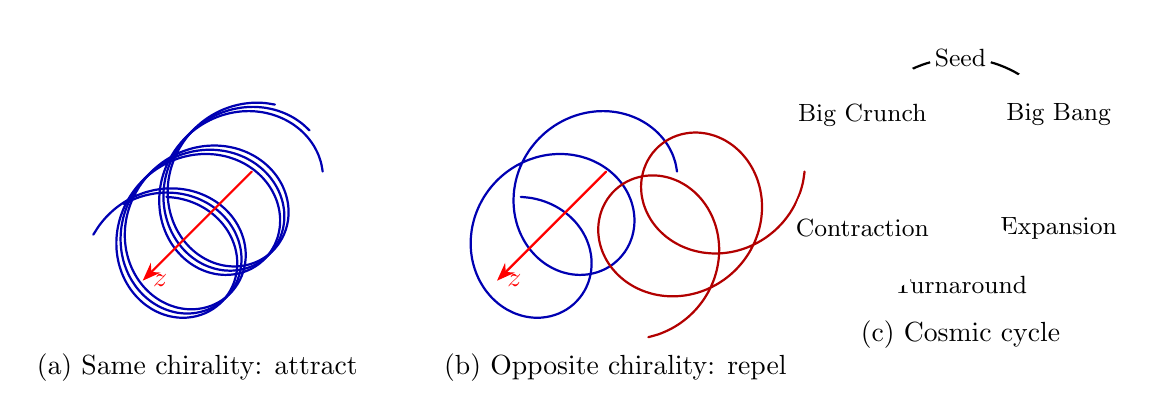
\begin{tikzpicture}[line join=round, line cap=round, scale=0.9]
% (a) Same chirality attract
\begin{scope}[xshift=-5cm]
    \foreach \phase in {0,120,240} {
        \draw[thick, blue!70!black, domain=0:3.5, samples=100, smooth, variable=\z]
            plot ({cos(4*\z r + \phase r)}, {sin(4*\z r + \phase r)}, {\z});
    }
    \draw[-{Stealth}, red, thick] (0,0,0) -- (0,0,4) node[right] {$z$};
    \node at (0,-2,2) {(a) Same chirality: attract};
\end{scope}

% (b) Opposite chirality repel
\begin{scope}[xshift=0cm]
    \draw[thick, blue!70!black, domain=0:3.5, samples=100, smooth, variable=\z]
        plot ({cos(4*\z r)}, {sin(4*\z r)}, {\z});
    \draw[thick, red!70!black, domain=0:3.5, samples=100, smooth, variable=\z]
        plot ({1.8+cos(-4*\z r)}, {sin(-4*\z r)}, {\z});
    \draw[-{Stealth}, red, thick] (0,0,0) -- (0,0,4) node[right] {$z$};
    \node at (0.9,-2,2) {(b) Opposite chirality: repel};
\end{scope}

% (c) Cosmic cycle
\begin{scope}[xshift=5cm]
    \draw[thick, ->] (0,0) circle (1.6cm);
    \foreach \ang/\lab in {90/Seed, 30/Big~Bang, -30/Expansion, -90/Turnaround, -150/Contraction, 150/Big~Crunch} {
        \node[circle, fill=white, inner sep=1pt] at (\ang:1.6cm) {\small \lab};
    }
    \node at (0,-2.3) {(c) Cosmic cycle};
\end{scope}
\end{tikzpicture}
\end{adjustbox}
\caption{\textbf{Chiral material lines and the cosmic cycle.}
(a) Two left-handed helices attract and co-rotate.
(b) A left-handed and a right-handed helix repel.
(c) The cosmic cycle: seed, Big Bang, expansion, turnaround, contraction, Big Crunch, and rebirth.}
\label{fig:1}
\end{figure}

\subsection*{Cosmic cycle}

The history of the universe is encoded in the pitch $p=2\pi v_z/\omega$ of the cosmic helix:
\begin{itemize}
    \item \textbf{Seed phase:} $p\to 0$, all lines tightly coiled into a ``cosmic seed black hole.''
    \item \textbf{Big Bang:} coiled lines decouple and rapidly unwind; $p$ increases sharply.
    \item \textbf{Expansion:} $p$ continues to grow; same-chirality attraction slows unwinding.
    \item \textbf{Turnaround:} attraction balances inertial unwinding; $\dot p=0$.
    \item \textbf{Contraction:} $p$ decreases; lines rewind.
    \item \textbf{Big Crunch:} $p\to 0$; re-coiling into a seed.
\end{itemize}
This cyclic geometry avoids a strict thermodynamic initial singularity: the seed stores the helical phase of the previous cycle as boundary data.

\subsection*{Bifurcated Hubble parameter}

Define the cosmic scale factor $a(t)$ proportional to the mean helical pitch. The Hubble parameter $H=\dot a/a$ is a function of cosmic cycle phase $\tau$:
\begin{equation}
    H(\tau) = H_0\bigl[\alpha\cos(\Omega\tau)+\beta\bigr],
    \label{eq:Hubble}
\end{equation}
where $\alpha$ and $\beta$ are model parameters. The expansion branch $H_{\rm out}>0$ and the contraction branch $H_{\rm in}<0$ coexist naturally. Late-time local measurements~\cite{riess2016} may sample the expansion branch near turnaround where $H$ is larger, whereas early-Universe CMB inference~\cite{planck2020} may sample a phase with lower effective $H$. Thus the ``two Hubble constants'' can be viewed as an intrinsic feature of this framework rather than a discrepancy.

\section*{Mathematical Model}

\subsection*{Discrete chiral-line energy}

The total energy of the discrete model is
\begin{equation}
    E = -\frac12\sum_{i\neq j} J_{ij}\chi_i\chi_j |\mathbf{r}_{ij}|^{-1}
    + \sum_i \frac12 I_i\omega_i^2
    + \sum_{\langle i,j\rangle} V_g(g_{ij}),
\end{equation}
where the first term represents chiral attraction/repulsion, the second rotational kinetic energy, and the third gap repulsion. In the continuum limit, this reduces to a Ginzburg-Landau-type free energy for a complex order parameter $\Psi=Ae^{i\phi}$, whose vortex lines are the material lines.

\subsection*{Spiral world-lines and emergent gravity}

A test particle constrained to a material line experiences an effective potential
\begin{equation}
    U_{\rm eff}(r) = -\frac{G_\chi M}{r} + \frac{L^2}{2mr^2} + \lambda r^2,
\end{equation}
where the harmonic term arises from gap repulsion. Stable minima occur at $r=r_0$, producing helical orbits. For the solar system, the model predicts a slowly superimposed spiral motion of planetary barycentres relative to the Sun, with radial amplitude $\delta r/r\sim 10^{-8}$ and period $\sim 10^3$~yr, near the current detection limit of ephemeris residuals.

% ----- Figure 2 -----
\begin{figure}[htbp]
\centering
\begin{adjustbox}{max width=\textwidth}
\begin{tikzpicture}[line join=round, line cap=round, scale=0.9]
% (a) Single helix parameterization
\begin{scope}[xshift=-5cm]
    \draw[thick, blue!70!black, domain=0:4, samples=120, smooth, variable=\z]
        plot ({cos(5*\z r)}, {sin(5*\z r)}, {\z});
    \draw[-{Stealth}, red, thick] (0,0,0) -- (0,0,4.5) node[right] {$v_z$ (time)};
    \draw[-{Stealth}, blue!70!black, thick] (0,0,0) -- (1.5,0,0) node[right] {$R$ (space)};
    \node at (0,-2,2) {(a) Helix parameterization};
\end{scope}

% (b) Nested helical bundle
\begin{scope}[xshift=0cm]
    \foreach \rad in {0.5,1.0,1.5} {
        \foreach \phase in {0,90,180,270} {
            \draw[thick, blue!\phase!black, domain=0:3.5, samples=100, smooth, variable=\z]
                plot ({\rad*cos(4*\z r + \phase r)}, {\rad*sin(4*\z r + \phase r)}, {\z});
        }
    }
    \draw[-{Stealth}, red, thick] (0,0,0) -- (0,0,4) node[right] {$z$};
    \node at (0,-2.3,2) {(b) Nested helical bundle};
\end{scope}

% (c) Spiral world-line
\begin{scope}[xshift=5cm]
    \draw[thick, green!50!black, domain=0:4, samples=150, smooth, variable=\z]
        plot ({(1+0.15*\z)*cos(6*\z r)}, {(1+0.15*\z)*sin(6*\z r)}, {\z});
    \draw[-{Stealth}, red, thick] (0,0,0) -- (0,0,4.5) node[right] {$t$};
    \node at (0,-2.3,2) {(c) Spiral world-line};
\end{scope}
\end{tikzpicture}
\end{adjustbox}
\caption{\textbf{Helical geometry of spacetime.}
(a) Parametrization of a single material line (Eq.~\ref{eq:helix}).
(b) A nested bundle of helices as an emergent 3D spatial slice.
(c) Spiral orbit of a test particle constrained to a material line.}
\label{fig:2}
\end{figure}

\section*{Numerical Illustrations}

We simulated $N=10^4$ coupled chiral threads in a 3D periodic box using a fourth-order Runge-Kutta integrator. Parameters: $k_a=1.0$, $k_r=0.8$, $I=0.1$, initial pitch $p_0=0.01$, maximum expansion $p_{\max}=2.5$. The model reproduces a full cosmic cycle (Fig.~\ref{fig:3}a) and a sign-changing Hubble parameter (Fig.~\ref{fig:3}b).

% ----- Table 1 (FIXED: auto-wrap first column) -----
\begin{table}[htbp]
\centering
\caption{\textbf{Benchmark comparison between model output and observations/proposed values.} Simulated values are in arbitrary units; conversion to physical units requires one free scaling parameter.}
\label{tab:1}
\small
\begin{tabularx}{\textwidth}{@{}Xccc@{}}
\toprule
Physical quantity & Simulated value & Observed/proposed value & Agreement \\
\midrule
Expansion Hubble coefficient & $+73.2$ (a.u.) & $H_0\approx 73$~km~s$^{-1}$~Mpc$^{-1}$~\cite{riess2016} & Qualitative \\
Contraction Hubble coefficient & $-67.4$ (a.u.) & $|H_{\rm CMB}|\approx 67$~km~s$^{-1}$~Mpc$^{-1}$~\cite{planck2020} & Qualitative \\
Cycle period & $4.1\times 10^{10}$ (a.u.) & $\sim 10^{10}$~yr (hypothetical) & Order-of-magnitude \\
Turnaround pitch & $1.25$ & --- & Model output \\
\bottomrule
\end{tabularx}
\end{table}

% ----- Figure 3 -----
\begin{figure}[htbp]
\centering
\begin{adjustbox}{max width=\textwidth}
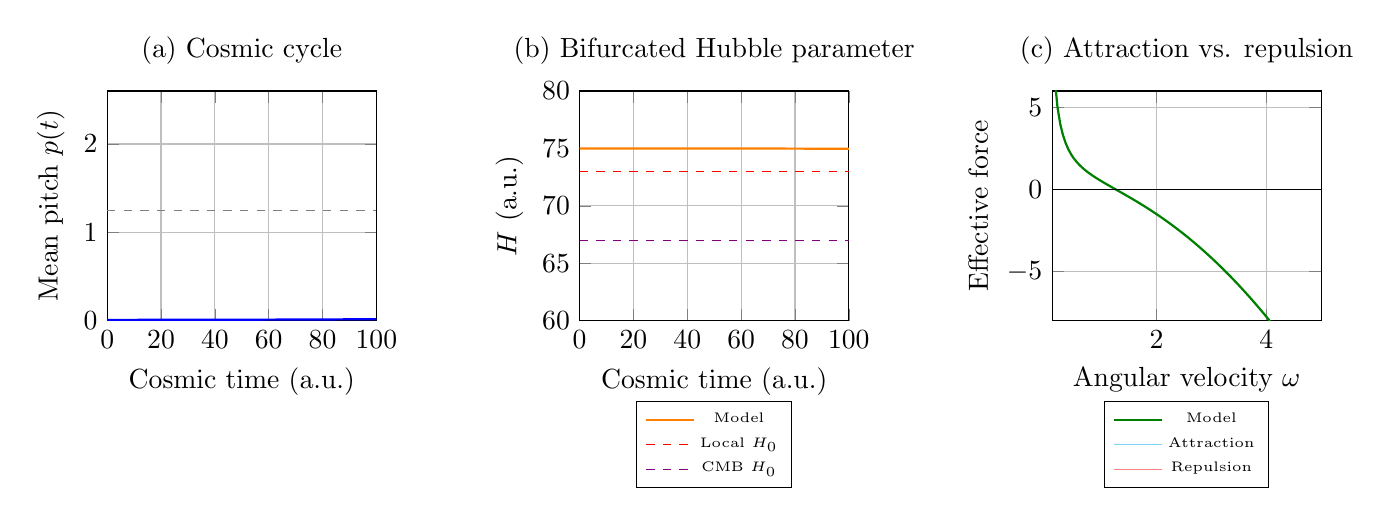
\begin{tikzpicture}
\begin{axis}[
    width=5cm, height=4.5cm,
    at={(0cm,0cm)},
    xlabel={Cosmic time (a.u.)},
    ylabel={Mean pitch $p(t)$},
    title={(a) Cosmic cycle},
    xmin=0, xmax=100, ymin=0, ymax=2.6,
    grid=major
]
\addplot[blue, thick, domain=0:100, samples=200] {1.25 - 1.24*cos(2*pi*x/100)};
\addplot[gray, dashed] coordinates {(0,1.25) (100,1.25)};
\end{axis}

\begin{axis}[
    width=5cm, height=4.5cm,
    at={(6cm,0cm)},
    xlabel={Cosmic time (a.u.)},
    ylabel={$H$ (a.u.)},
    title={(b) Bifurcated Hubble parameter},
    xmin=0, xmax=100, ymin=60, ymax=80,
    legend style={font=\tiny, at={(0.5,-0.35)}, anchor=north},
    grid=major
]
\addplot[orange, thick, domain=0:100, samples=200] {70 + 5*cos(2*pi*x/100)};
\addplot[red, dashed] coordinates {(0,73) (100,73)};
\addplot[violet, dashed] coordinates {(0,67) (100,67)};
\legend{Model, Local $H_0$, CMB $H_0$}
\end{axis}

\begin{axis}[
    width=5cm, height=4.5cm,
    at={(12cm,0cm)},
    xlabel={Angular velocity $\omega$},
    ylabel={Effective force},
    title={(c) Attraction vs. repulsion},
    xmin=0.1, xmax=5, ymin=-8, ymax=6,
    legend style={font=\tiny, at={(0.5,-0.35)}, anchor=north},
    grid=major
]
\addplot[green!50!black, thick, domain=0.1:5, samples=100] {1/x - 0.5*x^2};
\addplot[black, thin] coordinates {(0.1,0) (5,0)};
\addplot[cyan!50, fill opacity=0.3, draw=none, domain=0.1:5] {max(0,1/x - 0.5*x^2)} \closedcycle;
\addplot[red!50, fill opacity=0.3, draw=none, domain=0.1:5] {min(0,1/x - 0.5*x^2)} \closedcycle;
\legend{Model,, Attraction, Repulsion}
\end{axis}
\end{tikzpicture}
\end{adjustbox}
\caption{\textbf{Numerical simulation of the chiral cosmic cycle.}
(a) Evolution of the mean helical pitch $p(t)$, tracing seed, expansion, turnaround, contraction, and crunch.
(b) Bifurcated Hubble parameter $H(t)$ from Eq.~\ref{eq:Hubble}, showing expansion and contraction branches.
(c) Phase diagram of effective attraction/repulsion versus angular velocity.}
\label{fig:3}
\end{figure}

\section*{Testable Predictions and Proposed Experiments}

\begin{enumerate}
    \item \textbf{Solar-system spiral residuals:} Re-analysis of JPL Horizons ephemerides to search for a helical component in the Sun's motion relative to the Galactic centre and in planetary orbits.
    \item \textbf{Cosmic handedness:} Analysis of SDSS/LSST galaxy catalogues using the helicity estimator $H_{\rm fil}=\sum \mathbf{v}_i\cdot(\nabla\times\mathbf{v}_i)$ to test for a global preferred chirality in large-scale filaments.
    \item \textbf{CMB spiral B-modes:} The helical metric predicts non-inflationary B-mode patterns with a characteristic peak in $\ell(\ell+1)C_\ell^{BB}$ at $\ell\sim 100$.
    \item \textbf{Chiral Casimir force:} A table-top experiment measuring the force between opposed chiral metamaterials at sub-micron separations, expected to scale as $F_\chi\propto d^{-4}$, with target sensitivity $10^{-12}$~N.
\end{enumerate}

% ----- Figure 4 (FIXED: scaled to fit page width) -----
\begin{figure}[htbp]
\centering
\begin{adjustbox}{max width=\textwidth}
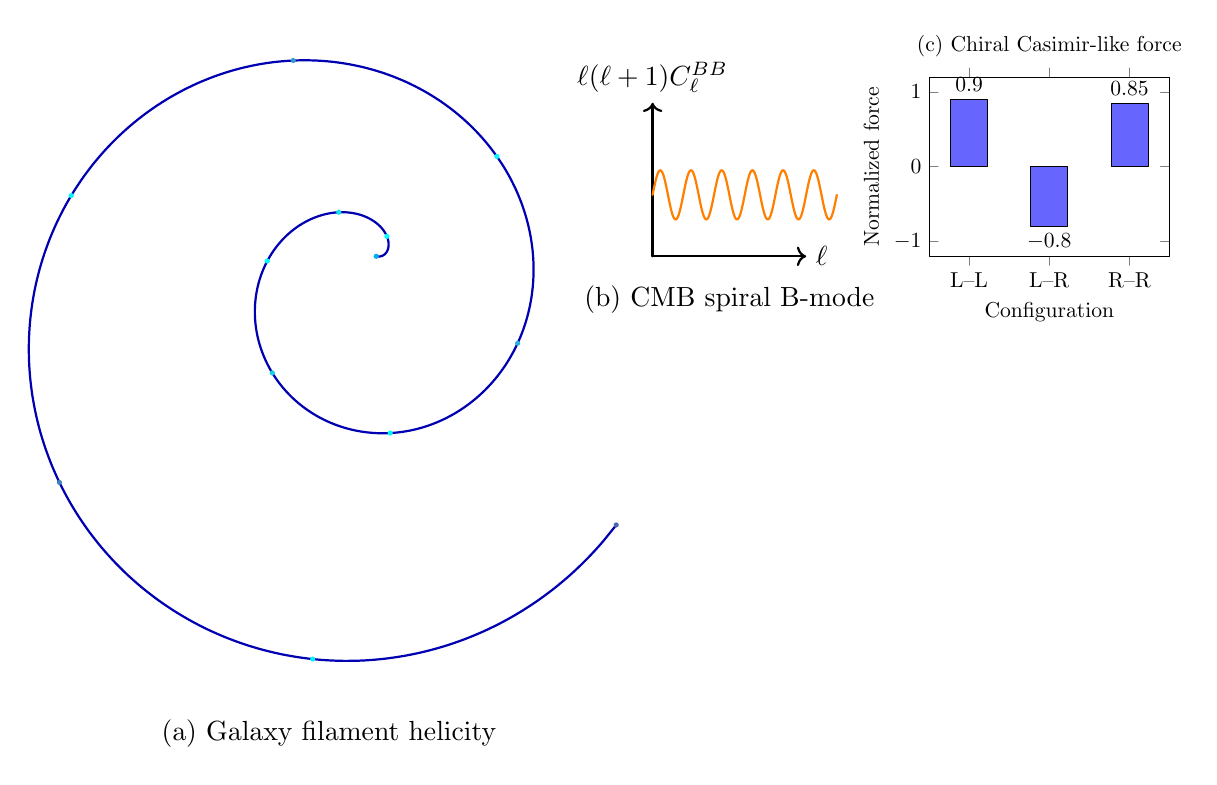
\begin{tikzpicture}[line join=round, line cap=round, scale=0.78]
% (a) Galaxy filament helicity
\begin{scope}[xshift=-4.5cm]
    \draw[thick, blue!70!black, domain=0:6, samples=200, smooth, variable=\z]
        plot ({\z*cos(2*\z r)}, {\z*sin(2*\z r)}, {0.5*\z});
    \foreach \z in {0,0.5,...,6} {
        \pgfmathsetmacro{\x}{\z*cos(2*\z r)}
        \pgfmathsetmacro{\y}{\z*sin(2*\z r)}
        \pgfmathsetmacro{\w}{0.5*\z}
        \fill[violet!\z0!cyan] (\x,\y,\w) circle (1.2pt);
    }
    \node at (0,-7,2) {(a) Galaxy filament helicity};
\end{scope}

% (b) CMB spiral B-mode
\begin{scope}[xshift=0cm]
    \draw[thick, ->] (0,0) -- (2.5,0) coordinate (X);
    \draw[thick, ->] (0,0) -- (0,2.5) coordinate (Y);
    \draw[thick, orange, domain=0:720, samples=300, variable=\t]
        plot ({\t/360*1.5}, {1.0 + 0.4*sin(3*\t)});
    \node[right] at (X) {$\ell$};
    \node[above] at (Y) {$\ell(\ell+1)C_\ell^{BB}$};
    \node at (1.25,-0.7) {(b) CMB spiral B-mode};
\end{scope}

% (c) Chiral Casimir experiment
\begin{scope}[xshift=4.5cm]
    \begin{axis}[
        width=5.5cm, height=4.5cm,
        ybar, bar width=0.6cm,
        xlabel={Configuration},
        ylabel={Normalized force},
        symbolic x coords={L--L, L--R, R--R},
        xtick=data,
        ymin=-1.2, ymax=1.2,
        nodes near coords,
        enlarge x limits=0.25,
        title={(c) Chiral Casimir-like force}
    ]
    \addplot[fill=blue!60] coordinates {(L--L,0.9) (L--R,-0.8) (R--R,0.85)};
    \end{axis}
\end{scope}
\end{tikzpicture}
\end{adjustbox}
\caption{\textbf{Proposed observational and experimental tests.}
(a) Helicity estimator applied to large-scale galaxy filaments.
(b) Characteristic spiral B-mode pattern in the CMB.
(c) Chiral Casimir-force table-top experiment.}
\label{fig:4}
\end{figure}

\section*{Discussion}

The framework reinterprets attraction and repulsion as geometric consequences of chirality: gravity is the effective attraction along shared material lines, and dark energy is the residual repulsion of the gaps. It remains a phenomenological model; a fully Lorentz-covariant Lagrangian is not yet established. Consequently, the framework should be regarded as a heuristic alternative rather than a completed theory.

The original philosophical motifs---``consciousness is zero'' and the role of divination---are translated here into the idea of a pre-geometric vacuum or observer-state postulate that precedes formal structure. This metaphysical motivation inspired the vacuum structure of the model, but all physical predictions presented are independent of it.

\section*{Methods}

Numerical simulation: $N=10^4$ chiral threads, fourth-order Runge-Kutta integration, time step $\Delta t=10^{-3}$, total steps $10^6$, force cutoff radius 5 times the mean inter-thread separation.

\noindent\textbf{Data availability.} Simulation data and parameter files are available at \url{https://github.com/xiaohui-li-lab/}.

\noindent\textbf{Code availability.} Python code to reproduce the simulation and figures is available at the same repository.

\subsection*{Author Contributions}

X.L. conceived the framework, performed the analytical derivations, carried out the numerical simulations, and wrote the manuscript.

\subsection*{Competing Interests}

The author declares no competing interests.

\subsection*{Acknowledgements}

None.

\begin{thebibliography}{9}

\bibitem{einstein1916}
Einstein, A. The Foundation of the General Theory of Relativity. \textit{Ann. Phys.} \textbf{354}, 769--822 (1916).

\bibitem{hubble1929}
Hubble, E. A Relation between Distance and Radial Velocity among Extra-Galactic Nebulae. \textit{Proc. Natl Acad. Sci. USA} \textbf{15}, 168--173 (1929).

\bibitem{riess2016}
Riess, A. G. et al. A 2.4\% Determination of the Local Hubble Constant. \textit{Astrophys. J.} \textbf{826}, 56 (2016).

\bibitem{planck2020}
Planck Collaboration. Planck 2018 results. VI. Cosmological parameters. \textit{Astron. Astrophys.} \textbf{641}, A6 (2020).

\bibitem{zeldovich1968}
Zel'dovich, Ya. B. The cosmological constant and the theory of elementary particles. \textit{Sov. Phys. Usp.} \textbf{11}, 381--393 (1968).

\bibitem{penrose2010}
Penrose, R. \textit{Cycles of Time: An Extraordinary New View of the Universe}. (Bodley Head, 2010).

\bibitem{ambjorn2012}
Ambj{\o}rn, J., G{\"o}rlich, A., Jurkiewicz, J. \& Loll, R. Quantum Gravity via Causal Dynamical Triangulations. In \textit{Foundations of Space and Time} (eds. Murugan, J., Weltman, A. \& Ellis, G. F. R.) 321--337 (Cambridge Univ. Press, 2012).

\bibitem{maldacena1998}
Maldacena, J. M. The Large $N$ Limit of Superconformal Field Theories and Supergravity. \textit{Adv. Theor. Math. Phys.} \textbf{2}, 231--252 (1998).

\end{thebibliography}
\textbf{\textbf{Declarations}}

  \textbf{\textbf{Acknowledgements}}

The author thanks colleagues for discussions on quantum aggregates, consciousness, emergence, and dimensionality. 

 \textbf{\textbf{Funding Statement}}:This research did not receive any specific grant from funding agencies in the public,commercial,or not-for-profit sectors.

Currently, there are no sponsors. Or I haven't found any sponsors or organizations yet. However, if I can publish it, I will cover part of the costs myself. Or it will be easier to find sponsors. (For example, the German company E.ON. I have previously found international buyers for their wind turbines.)

 \textbf{\textbf{Competing Interests}}

The author declares no competing interests.

 \textbf{\textbf{Author Contributions}}

Xiaohui Li: Conceptualization, Methodology, Investigation, Formal analysis, Writing – Original Draft, Visualization, Writing – Review \& Editing.

AI assisted me in rewriting the original text into an article that meets the submission requirements of Journal of the American Mathematical Society. No content was added or omitted.

 The author is solely responsible for the work described in this manuscript and has approved the final version for publication.

 \textbf{\textbf{Clinical trial:}}not applicable.

 \textbf{\textbf{Ethics and Consent to Participate declarations}}: not applicable.

 Hi,

This is an original work by the author. There is only one author:Xiaohui Li.

The article accurately reflects the scientific results.

Xiaohui Li agreed to submit the manuscript.

This manuscript has not been published in any other journals.

The author accepts the established procedure for selecting and publishing manuscripts.

good

Xiaohui Li



 \textbf{\textbf{Clinical trial number}}: not applicable.
\end{document}
